\chapter{The random projection method}
\label{chap:rp-method}

In this chapter we present the proposed method in detail and discuss its constructive elements. First, we explain the central idea behind our proposal in section \ref{sec:method_idea} and provide a brief overview of the theory behind random projections. In section \ref{sec:method_elements}, we proceed with a study of the critical elements that together compose the random projection method for reconstruction-based outlier detection. We conclude with the final formulation of the method in section \ref{sec:method_formulation}.

\section{Making use of random projections}
\label{sec:method_idea}
In this section we go through the main idea behind our method and discuss the lemma standing at the basis of our hypothesis. We also explain the variants of methods to generate random projection directions as found in the literature, and which variant we implement.

\subsection{The idea}
As already explained in the previous chapters, the PCA-based reconstruction method for outlier detection is closely related to our method. More specifically, instead of projecting the data into the principal directions and make all computational efforts to obtain those directions online, we simply project the data in random directions and hope for the best. 

Obviously, projecting the data into random directions takes away the computational burden associated with outlier detection methods based on PCA or other data-dependent methods. Another beneficial property is that we only need to set one parameter: the number of projection vectors $k$. With these two properties of random projections, we attempt to address the two main shortcomings of SPIRIT in the light of the challenges. Figure \ref{fig:method_geometry_rp} illustrates the geometrical difference between projecting the data into the (first) principal direction and a random direction. 

\begin{figure}[h]
	\centering
	\includegraphics[scale=1.8]{rp-method/geometry_projections_rp1}
	\caption{Geometrical representation of a projection into the first principal (left) and a random direction (right).}
	\label{fig:method_geometry_rp}
\end{figure}

This random model likely enables reconstruction of the outliers to some extent, but the squared Euclidean distance between a reconstructed outlier and its original version is still assumed to be higher than for the normal data points. Therefore, we hypothesize that a less perfect model than resulting from the principal components might still be sufficient in order to interpret the reconstruction errors as outlier scores. It might be the case, that we need more random projection vectors to obtain a reasonable model that approaches the model obtained by PCA-based methods. Hypothesis \ref{hyp:method_foundation} formulates this idea more formally.

\vspace{0.2cm}
\begin{hypothesis}\label{hyp:method_foundation}
	Replacing the $k_{\text{pca}}$ principal coefficient vectors with $k_{\text{rp}}$ random coefficient vectors, where $k_{\text{pca}} < k_{\text{rp}}$, yields a similar model of the normal behaviour at a lower computational cost.
\end{hypothesis}
\vspace{0.2cm}

The principle underlying our idea is a lemma posed by Johnson and Lindenstrauss in 1984 \cite{johnson1984extensions}. They state that, given a data set $\mathbf{X}$ of size $d \times n$ there exists a linear mapping $\mathbf{f}$ to obtain a $k$-dimensional representation of $\mathbf{X}$ with $k \ll d$, such that with high probability the pair-wise (squared) Euclidean distances are preserved with distortion at most $\varepsilon$. See also lemma \ref{lemma:onelemma}.

\vspace{0.2cm}
\begin{lemma}\label{lemma:onelemma}
	(Johnson and Lindenstrauss \cite{johnson1984extensions}). Given $\varepsilon > 0$ and an integer $n$, let $k$ be a positive constant $k \geq \mathcal{O}(\frac{1}{\varepsilon^2}\log(n))$. Then, for an arbitrary data set ${\mathbf X}$ of $n$ data points ${\mathbf x} \in \mathbb{R}^d$, there exists an $\mathbf{f}$ : ${\mathbb R}^d \rightarrow {\mathbb R}^k$ such that for all pairs ${\mathbf x}, {\mathbf y} \in {\mathbf X}$:
	\[(1-\varepsilon)\|{\mathbf x} - {\mathbf y}\|^2 \leq \|\mathbf{f}({\mathbf x}) - \mathbf{f}({\mathbf y})\|^2 \leq (1+\varepsilon)\|{\mathbf x} - {\mathbf y}\|^2 \]
	with probability $1-\frac{1}{n^2}$.
\end{lemma}
\vspace{0.2cm}

Note that the projection dimensionality $k$ only depends on the number of data points $n$ in $\mathbf{X}$ and the allowed distortion $\varepsilon$, and not on the original dimensionality $d$. For example, if we want to represent $n=500$ data points in $\mathbb{R}^d$ with at most $\varepsilon = 0.1$ distortion we would need $k$ to be approximately $\frac{2}{0.1^2}\log(n) \approx 540$ according to the bound empirically found sufficient for most variants of $\mathbf{f}$ by Venkatasubramanian et al. \cite{venkatasubramanian2011johnson}. This implies that, irrespective of the original dimensionality $d$, we can represent all $500$ data points in a $540$-dimensional subspace while retaining the pair-wise distances properly. Obviously, this would only make sense if $d > 540$. 

The topic of what we can and should use for $\mathbf{f}$ has been studied a lot over the past years since dealing with high-dimensional data sets has received increasing interest as emphasized already in chapter \ref{chap:introduction}.
The most important work has been devoted to finding suitable mappings that reduce the presented lower bound on $k$, or to improve the computational effort associated with it. 

\vspace{0.3cm}
\subsection{Variants of $\mathbf{f}(\mathbf{x})$}

In the literature a large variation of methods can be found for obtaining a lower-dimensional representation of $\mathbf{X}$ using random projections, here we briefly present the most important developments. As mapping $\mathbf{f}$ is linear, we define it as a random matrix $\mathbf{R}$ and refer to it as the random projection matrix representing this mapping. Then, we can define $\mathbf{f}(\mathbf{x})$ by the matrix multiplication

\vspace{0.1cm}
\begin{equation}
	\mathbf{f}(\mathbf{x}) = \mathbf{R}\mathbf{x}.
\end{equation}

Johnson and Lindenstrauss initialized the study to random projections and proposed a first method for obtaining $\mathbf{R}$. They sampled each entry $r$ of $\mathbf{R}$ from the Gaussian distribution with $0$ mean and unit variance, i.e. $r \sim \mathcal{N}(0,1)$. The resulting projection matrix should then be orthogonalized to meet the conditions they found to be necessary:

\begin{itemize}
	\item Spherical symmetry: For any orthogonal matrix $\mathbf{X} \in \mathbb{R}^{d \times n}$, the entries in $\mathbf{R} \mathbf{X}$ and $\mathbf{R}$ follow the same distribution.
	\item Orthogonality: All $k$ projection vectors in $\mathbf{R}$ are orthogonal to each other.
	\item Normality: All $k$ projection vectors in $\mathbf{R}$ are of unit length \cite{ailon2009fast}.
\end{itemize}

Random projections are particularly useful if we want to avoid the computational burden of obtaining a qualitative lower-dimensional representation of a data set $\mathbf{X}$. Instead of optimizing this lower-dimensional representation, by making use of random projections we obtain a representation that solely preserves pair-wise distances, yet in a more efficient manner. Therefore, the need for orthogonalizing $\mathbf{R}$ is considered a bottleneck, especially if $d$ is high. Indyk and Motwani \cite{indyk1998approximate} significantly improved the computational complexity by drawing the entries $r$ of $\mathbf{R}$ from a normal distribution with $0$ mean and $\frac{1}{d}$ variance, which is equivalent to scaling a matrix $\mathbf{R}$ with $r \sim \mathcal{N}(0,1)$ with $\frac{1}{\sqrt{d}}$. Scaling $\mathbf{R}$ this way makes it orthonormal on expectation. The higher $d$ gets, the closer the resulting projection matrix approaches orthonormality. Technically speaking, $\mathbf{R}$ is only a projection matrix if it is strictly orthogonal, which obviously is not the case if it is orthogonal on expectation. For the sake of simplicity we ignore this for the remainder of this work, and slightly abuse terminology by referring to this approximately orthogonal linear mapping as an approximately orthogonal linear projection.

\vspace{0.2cm}
Following the desire of relaxing the necessity conditions for $\mathbf{R}$ as posed by Johnson and Lindenstrauss, Achlioptas \cite{achlioptas2003database} noticed that the spherical symmetry condition of $\mathbf{R}$ could be dropped as well. Instead of sampling all entries from Gaussian distributions resulting in dense but spherical symmetric projection matrices, we might as well sample from the simple distribution $\{-1,+1\}$ where each element is drawn equally likely. The operations needed to project $\mathbf{X}$ onto $\mathbf{R}$ then solely consist of summations and subtractions, which speeds up the computations. Another significant contribution by Achlioptas is the proposal of sampling the entries from a sparse distribution $\{-1,0,+1\}$. In that case, we can store $\mathbf{R}$ as a sparse matrix saving storage, where the number of operations needed to be done to project data points would be reduced at the same time. 

Several improvements and (advanced) alternatives for $\mathbf{R}$ followed \cite{li2006very,ailon2009fast,krahmer2011new,clarkson2013low}, resulting in even lower storage requirements, less projection vectors required or mathematical operations needed.
It depends on the structure of the data set at hand whether such more efficient (possibly sparse) random projection methods properly preserve its pair-wise distances. For example, if the data set is sparse, a sparse random projection matrix might not properly preserve pair-wise distances \cite{venkatasubramanian2011johnson}. 

\vspace{0.2cm}
\section{Fundamental building blocks}
\label{sec:method_elements}

As we do not assume a certain structure on the data stream, we simply adopted the conventional dense Gaussian version for $\mathbf{R}$ with entries $r \sim \mathcal{N}(0,1)$ which was shown to be suitable for differently structured data sets. To bypass the expensive orthogonalization procedure, we scale our matrix as proposed by Indyk and Motwani \cite{indyk1998approximate}. 
Even though it often is not made explicit, it is important to scale the resulting projection with an additional factor $\sqrt{\frac{d}{k}}$ if one is concerned with preserving the original pair-wise Euclidean distances \cite{bingham2001random}. The reason behind this, is that the norms of the projections are down-scaled to $\sqrt{\frac{k}{d}}\|\mathbf{x}_i\|$ on expectation. To compensate for this effect, we could project $\mathbf{x}_i$ following

\vspace{0.1cm}
\begin{equation}\label{method_scaled_projection}
	\mathbf{x}_i' = \sqrt{\frac{d}{k}} \frac{1}{\sqrt{d}} \mathbf{R} \mathbf{x}_i.
\end{equation}
\vspace{0.1cm}

It is not hard to imagine that we could simplify this by scaling $\mathbf{R}$ directly with $\frac{1}{\sqrt{k}}$, which indeed seems to be a nice short-cut. The use of this short-cut as being interchangeable with the scaling factors used in equation \eqref{method_scaled_projection} can be found scattered throughout the literature \cite{arriaga1999algorithmic,achlioptas2003database,fradkin2003experiments}. Aside from the literature, this scaling method is frequently implemented by default in toolboxes such as scikit-learn \cite{scikit2018random}. We could blindly adopt this short-cut scaling method, but the success of our reconstruction-based method strongly coheres with the way projection matrix $\mathbf{R}$ is constructed. It also seems important to question to what extent we can use a projection matrix that is only orthonormal on expectation in order to use the cheap reconstruction method as in equation \eqref{eq:reconstruction_pcareconstruction}.

To evaluate these aspects of our method, we started investigating both scaling options to see if, and how well, they preserve the pair-wise Euclidean distances compared to a strictly orthonormal projection basis. To do so, we used a random data set of size $n = 997$ by $d = 300$. Figure \ref{fig:distortion_distances} shows how both scaling methods evidently result in the same distortion fraction of the pair-wise Euclidean distances. In addition, it can be seen that this data set could be qualitatively represented in a subspace of lower dimensionality than empirically found sufficient for most data sets as in \cite{venkatasubramanian2011johnson}. Finally, from this figure we can conclude that both scaling methods approach the distortion of the pair-wise distances as resulting from the strictly orthogonal projection matrix. 

\begin{figure}[h]
	\centering
	\vspace{-0.1cm}
	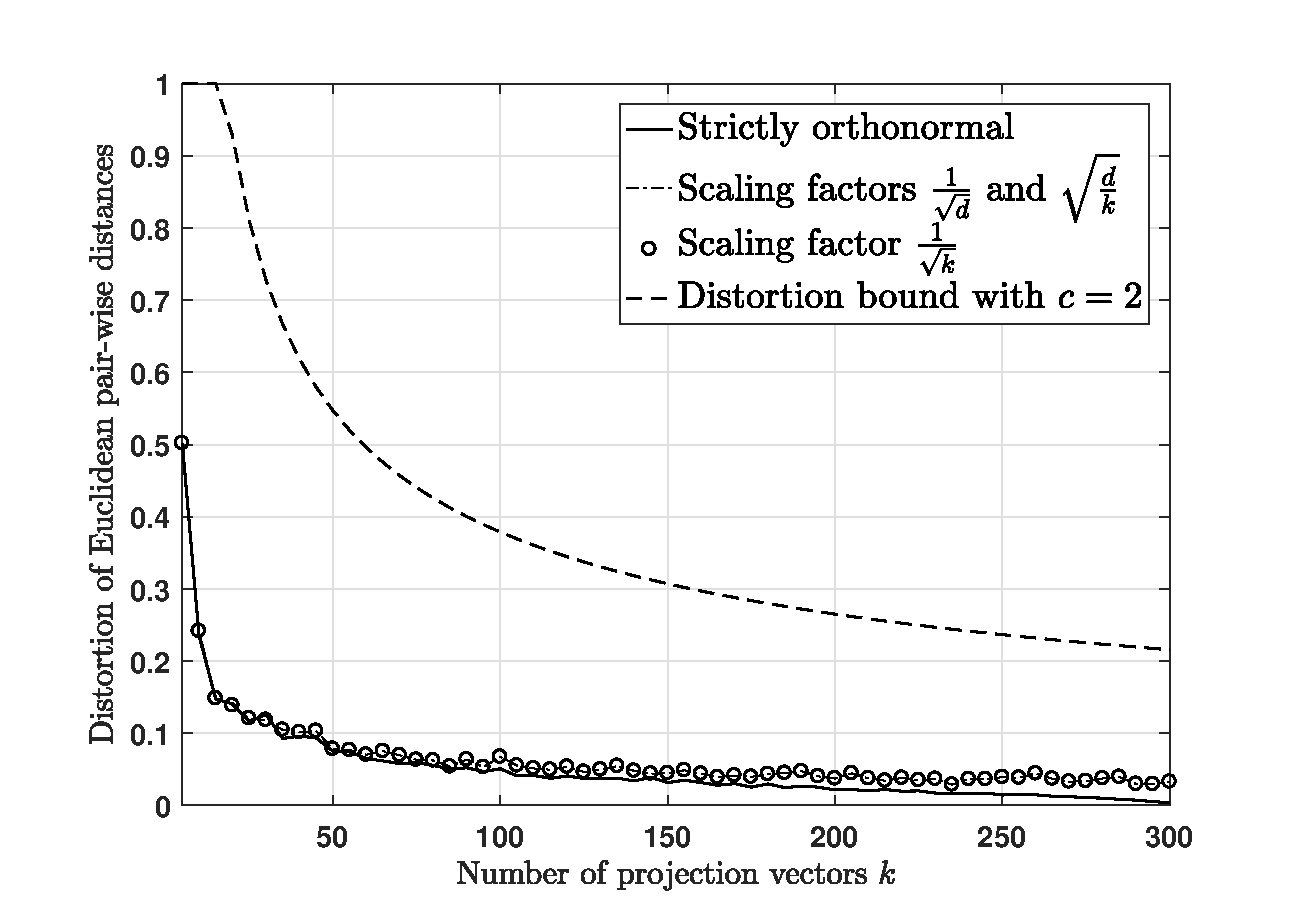
\includegraphics[scale=0.4]{rp-method/Distortion_distances}
	\vspace{-0.1cm}
	\caption{Distortion of pair-wise distances obtained by the different projection matrices and the bound on $\varepsilon$ from $k=(\frac{2}{\varepsilon^2} \ \log(n))$ \cite{venkatasubramanian2011johnson}.}
	\label{fig:distortion_distances}
\end{figure}

\newpage
However, in order to make the cheap reconstruction method as in equation \eqref{eq:reconstruction_pcareconstruction} possible, the approximately orthogonal projection vectors in $\mathbf{R}$ must be of unit length as well. To that end, figure \ref{fig:average_norms} shows that the average norm of the projection vectors with scaling factor $\frac{1}{\sqrt{k}}$ is on expectation equal to $\sqrt{\frac{d}{k}}$ instead of $1$. The norm of this projection matrix only approaches $1$ if $k$ approaches $d$. This implies that $\frac{1}{\sqrt{k}} \mathbf{R}^T \ \frac{1}{\sqrt{k}} \mathbf{R} \not\approx \mathbf{I}$ with $r \sim \mathcal{N}(0,1)$. Hence, we cannot use this short-cut in our method.

\begin{figure}[h]
	{\centering
		\vspace{-0.1cm}
		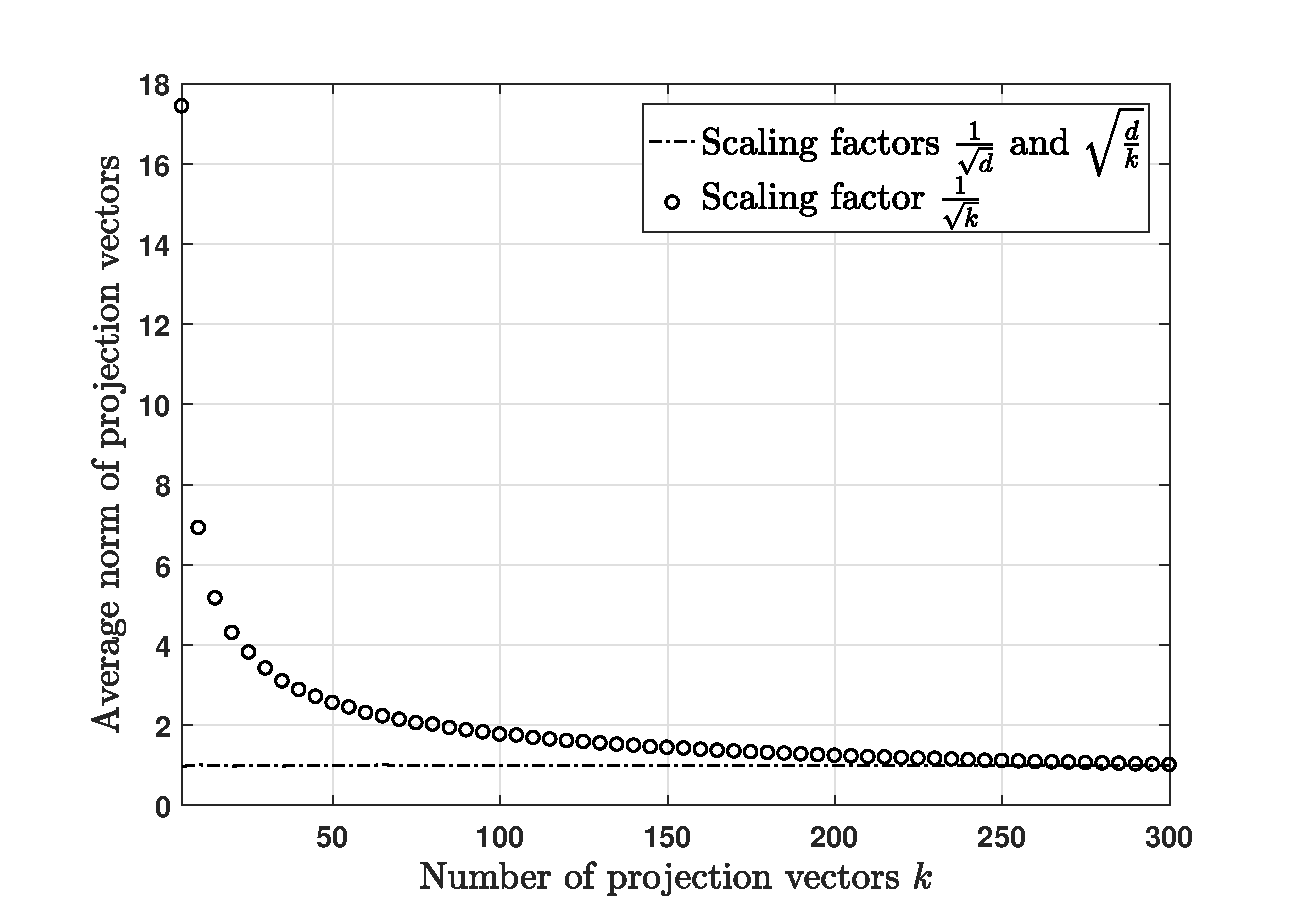
\includegraphics[scale=0.4]{rp-method/Norms_projection_vectors}
		\vspace{-0.1cm}
		\caption{Average norms of the $k$ projection vectors for $k$ ranging from $1$ to $d$.}
		\label{fig:average_norms}}
\end{figure}

Two questions remain open ended. First, how well can we reconstruct a projected vector using the cheap reconstruction method (taking the transpose $\mathbf{R}^T$ instead of the inverse $\mathbf{R}^{-1}$) from a projection matrix that is only orthonormal on expectation? Going from the following observations:

\begin{itemize}
	\itemsep0em
	\item the pair-wise Euclidean distances preserved are almost equal to the distances preserved using strictly orthogonal projection vectors as shown in figure \ref{fig:distortion_distances},
	\item the average norms of the $k$ projection vectors are very close to $1$ for $k = 1$ already, and
	\item the product $\frac{1}{\sqrt{d}}\mathbf{R}^T \ \frac{1}{\sqrt{d}}\mathbf{R}$ approximates $\mathbf{I}$ closely,
\end{itemize}

\noindent it might depend on the choice for $k$ and the original dimensionality $d$, but we have confidence it will bring the desired reconstruction results in most cases. Therefore, we will scale $\mathbf{R}$ with $r \sim \mathcal{N}(0,1)$ by the factor $\frac{1}{\sqrt{d}}$ resulting in orthonormality only on expectation, but still use the cheap reconstruction method.

The final unanswered question is whether we should care about the norm of the projection $\mathbf{x}_i'$ being scaled down with $\sqrt{\frac{k}{d}}$ on expectation? If so, at what point should we then scale it back with $\sqrt{\frac{d}{k}}$?
For separability purposes it does not make a difference if the reconstruction approaches the original data point or not as also noted in \cite{fradkin2003experiments}. Yet, for our method it is an important consideration as we actually use the difference between the reconstruction of $\mathbf{x}_i'$ as well as the original data point $\mathbf{x}_i$ to derive the outlier scores.

First, let us determine where scaling with $\sqrt{\frac{d}{k}}$ would be in place. If we would scale the projection $\mathbf{x}_i'$ of $\mathbf{x}_i$ before reconstruction, we basically reconstruct a transformed version of the original projection. For the sake of proper reconstruction, we need $\mathbf{x}_i'$ to be the original projection of $\mathbf{x}_i$. Therefore, the reconstruction $\hat{\mathbf{x}}_i$ of $\mathbf{x}_i'$ should be scaled instead, to obtain a reconstruction of which the norm ($\|\hat{\mathbf{x}_i}\|$) approximates the norm of the original data point ($\|\mathbf{x}_i\|$). To illustrate the effect of scaling the reconstruction back, figure \ref{fig:effect_backscaling} shows the difference between an example time series $\mathbf{x}_j$, its unscaled reconstruction and scaled reconstruction\footnote{The presented time series is just $1$ out of $60$ time series with random phase, amplitude, offset and noise, which causes the misalignment between the original and its reconstructions.}.

\begin{figure}[h]
	{\centering
		\vspace{-0.32cm}
		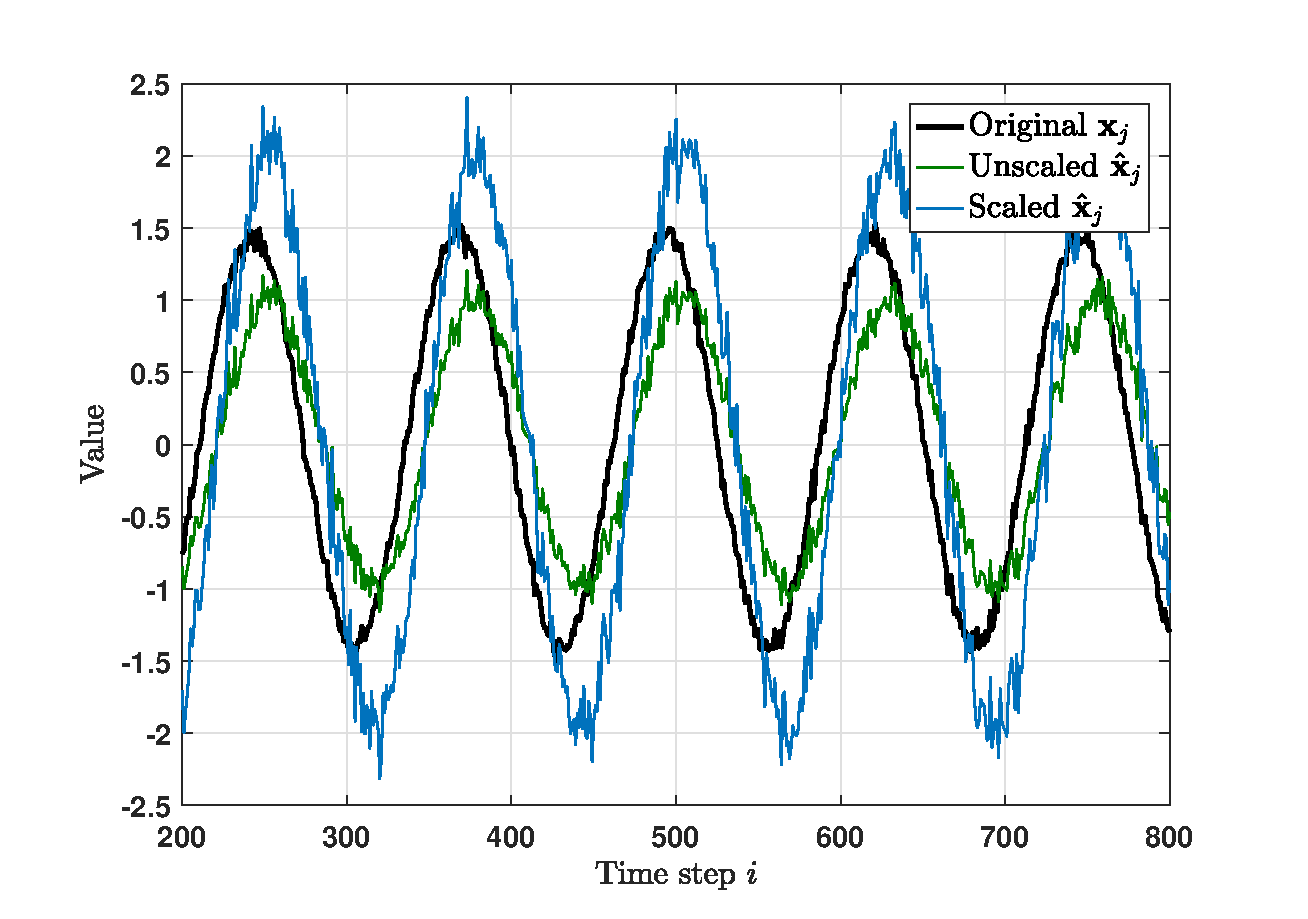
\includegraphics[scale=0.38]{rp-method/Effect_reconstruction_backscaling1}
		\vspace{-0.3cm}
		\caption{Effect of scaling the reconstruction back with $\sqrt{\frac{d}{k}}$.}
		\label{fig:effect_backscaling}}
		\vspace{-0.2cm}
\end{figure}

As can be derived from this figure, whether back-scaling improves our model for detection purposes is tightly associated with the type of outliers to be found in the data. Starting with global point outliers it seems better to use the unscaled reconstruction, as we will discriminate outliers that are far from the model by making use of the squared Euclidean distance between $\mathbf{x}_i$ and $\hat{\mathbf{x}_i}$. So, in that case we do not want our model to be closer to the original values as results from scaling the reconstructed version back with $\sqrt{\frac{d}{k}}$. This becomes clear if we consider the time series as in figure \ref{fig:effect_backscaling} and imagine a global point outlier appearing around $i=500$ (e.g. its value is around $2$ instead of $1.5$). Then the squared Euclidean distance between $\mathbf{x}_i$ and $\sqrt{\frac{d}{k}} \ \hat{\mathbf{x}}_i$ would be smaller compared to all normal data points instead of larger. The unscaled reconstruction does not suffer from this.

On the contrary, to find contextual outliers we want a model close to the original and hope it is indeed very close to the original without modelling any outliers. Considering the same example at $i=500$ but instead with its value around $1$ instead of $1.5$. We would be better off back-scaling the resulting reconstruction as we get a higher squared Euclidean distance between the model and the original point for contextual outliers.
As the success of back-scaling might depend on the data at hand, we assessed its actual influence on the outlier detection performance experimentally in chapter \ref{chap:analysis}. 

Beside the influence of the scaling factors on the outlier detection performance, our lower-dimensional representations and reconstructions are close to the mean and average range of all time series together. This implies that our method is sensitive to the mean and range of the input data. Hence, it is preferable to estimate the mean (and possibly standard deviation) of the different time series online to correct for this effect. As such online parameter estimations might not be accurate enough, we analysed the performance for standardized data such that each time series has $0$ mean and unit variance, and data of which the means and ranges are approximately equal.


\section{The proposed method}
\label{sec:method_formulation}

Altogether, the mathematical procedures to compute the projection, reconstruction and outlier score of a data point $\mathbf{x}_i$ online are quite similar to the procedures presented in chapter \ref{chap:reconstruction-detection}. That is, we obtain our projection by

\vspace{-0.2cm}
\begin{equation}\label{eq:method_projection}
\mathbf{x}_i' = \frac{1}{\sqrt{d}} \mathbf{R} \ \mathbf{x}_i
\end{equation}

\noindent where $\mathbf{R}$ is the random coefficient matrix of size $k \times d$ with entries $r \sim \mathcal{N}(0,1)$. Then the projected data point $\mathbf{x}_i'$ is easily reconstructed to its original dimensionality $d$ using

\vspace{-0.1cm}
\begin{equation}\label{eq:method_reconstruction}
\hat{\mathbf{x}}_i = \frac{1}{\sqrt{d}} \mathbf{R}^T \ \mathbf{x}_i'
\end{equation}  

\noindent where $\mathbf{R}^T$ is used instead of the inverse $\mathbf{R}^{-1}$ as we have 

\vspace{-0.1cm}
\begin{equation}\label{eq:method_orthonormality}
\frac{1}{\sqrt{d}} \mathbf{R}^T \ \frac{1}{\sqrt{d}} \mathbf{R} \approx \mathbf{I}.
\end{equation}  

Finally, as mentioned in the previous section, it depends on the data (and outliers) and the quality of the projections and reconstructions if back-scaling results in a more accurate model close to the original data point. For the sake of completeness, if one wants a reconstruction closer to the original data point, we need to scale the reconstruction by

\vspace{-0.1cm}
\begin{equation}\label{eq:method_scaledreconstruction}
\hat{\mathbf{x}}_i \gets \sqrt{\frac{d}{k}} \ \hat{\mathbf{x}}_i
\end{equation} 

\noindent The outlier score $O_i$ is computed similarly as in equation \eqref{eq:reconstruction_score}. Each outlier score should then be converted to an actual binary label (e.g. $0$ for normal data points and $1$ for outliers). To do so, a threshold $\theta$ should be set such that if $O_i \leq \theta$ the corresponding data point is labelled as normal else as an outlier. Eventually, we want $\theta$ to minimize the error between all the predicted and actual labels\footnote{Misclassified outliers might be more costly than misclassified normal data points or vice versa, therefore $\theta$ actually optimizes the weighted balance between these two. This is explained in chapter \ref{chap:analysis}.}. Algorithm \ref{alg:analysis_algorithm} presents the final algorithm we propose.

\vspace{-0.2cm}
\begin{algorithm}[H]
	\vspace{-0.1cm}
	\caption{\quad \textbf{RP}}
	\label{alg:analysis_algorithm}
	\begin{flushleft}
		\vspace{-0.2cm}
		\textbf{Input} data point $\mathbf{x}_i$ of size $d \times 1$\\	
		\textbf{Input} number of projection vectors $k$	
		\vspace{-0.1cm}
	\end{flushleft}
	\begin{algorithmic}[1]
		\vspace{-0.2cm}
		\IF{$i=1$}
			\STATE Generate ${\mathbf R}$ of size $k \times d$ with entries $r \sim \mathcal{N}(0,1)$
		\ENDIF
			\STATE Project $\mathbf{x}_i$ on $\mathbf{R}$ by ${\mathbf x}_i' = \frac{1}{\sqrt{d}} {\mathbf R} \ {\mathbf x}_i$ 
			\STATE Reconstruct ${\mathbf x}_i'$ to $\hat{{\mathbf x}}_i = \frac{1}{\sqrt{d}} {\mathbf R}^T \ {\mathbf x}_i'$
		\IF{approximate norm preservation is desired}
			\STATE Scale reconstruction back $\hat{\mathbf{x}}_i = \sqrt{\frac{d}{k}} \hat{\mathbf{x}}_i$
		\ENDIF
		\STATE $O_i = \|{\mathbf x}_i - \hat{{\mathbf x}}_i\|^2$
	\end{algorithmic}
	\begin{flushleft}
		\vspace{-0.3cm}
		\flushleft\textbf{Output} outlier score $O_i$
	\end{flushleft}
\end{algorithm}
\vspace{-0.2cm}

To deploy the RP method for outlier detection in multivariate time series, we just need to generate $\mathbf{R}$ once at the start of the stream $\mathbf{X}$. From there, we only need $2$ matrix-vector multiplications resulting in a runtime of $\mathcal{O}(kd)$ per data point as well. Though it seems close to $\mathcal{O}(k^2d)$, it depends quadratically on $k$ and the constant hidden in this upper bound associated with SPIRIT is higher. If we consider, for instance, algorithms \ref{alg:spirit} and \ref{alg:trackw} it becomes clear that SPIRIT conducts more matrix-vector multiplications to update the principal coefficient matrix $\mathbf{W}$ than needed with the RP method. In chapter \ref{chap:analysis} we experimentally explored the behaviour of the runtime of SPIRIT for varying values of $d$ and $k$.

